It has been more than 30 years, since it was proven, that already simple neural network architectures can in fact be \emph{universal approximators} \cite*{ffnUnversalApproximator}. 
That means that if a problem can be formulated as a mathematical function, this function can be approximated by a neural network.
This has huge consequences, because if input and output are encoded digitally in a predefined format, \emph{all} mappings between these can be formulated in form of a mathematical function. 
Be it only the trivial one, that maps each input encoding to the desired output encoding.
Because of that, seemingly impossibly complex problems can be tackled now days. 

Part of the experimentation in the thesis will focus on the application of a select breed of neural networks on the \emph{image classification task}.
This is not a novel problem, but one that has been triad and soled by many teams of researchers. 
The gist is, to build a neural network that can label the things pictured on some kind of image.
In our case, an even simpler version of the problem will be considered. 
The only job of the network is, to select one of $N$ predefined labels, that describe the picture best.

The architecture of the network can be viewed generalized in \autoref{fig:immage-classification-general}.

\begin{figure}[htbp]
    \centering
    \makebox[\textwidth][c]{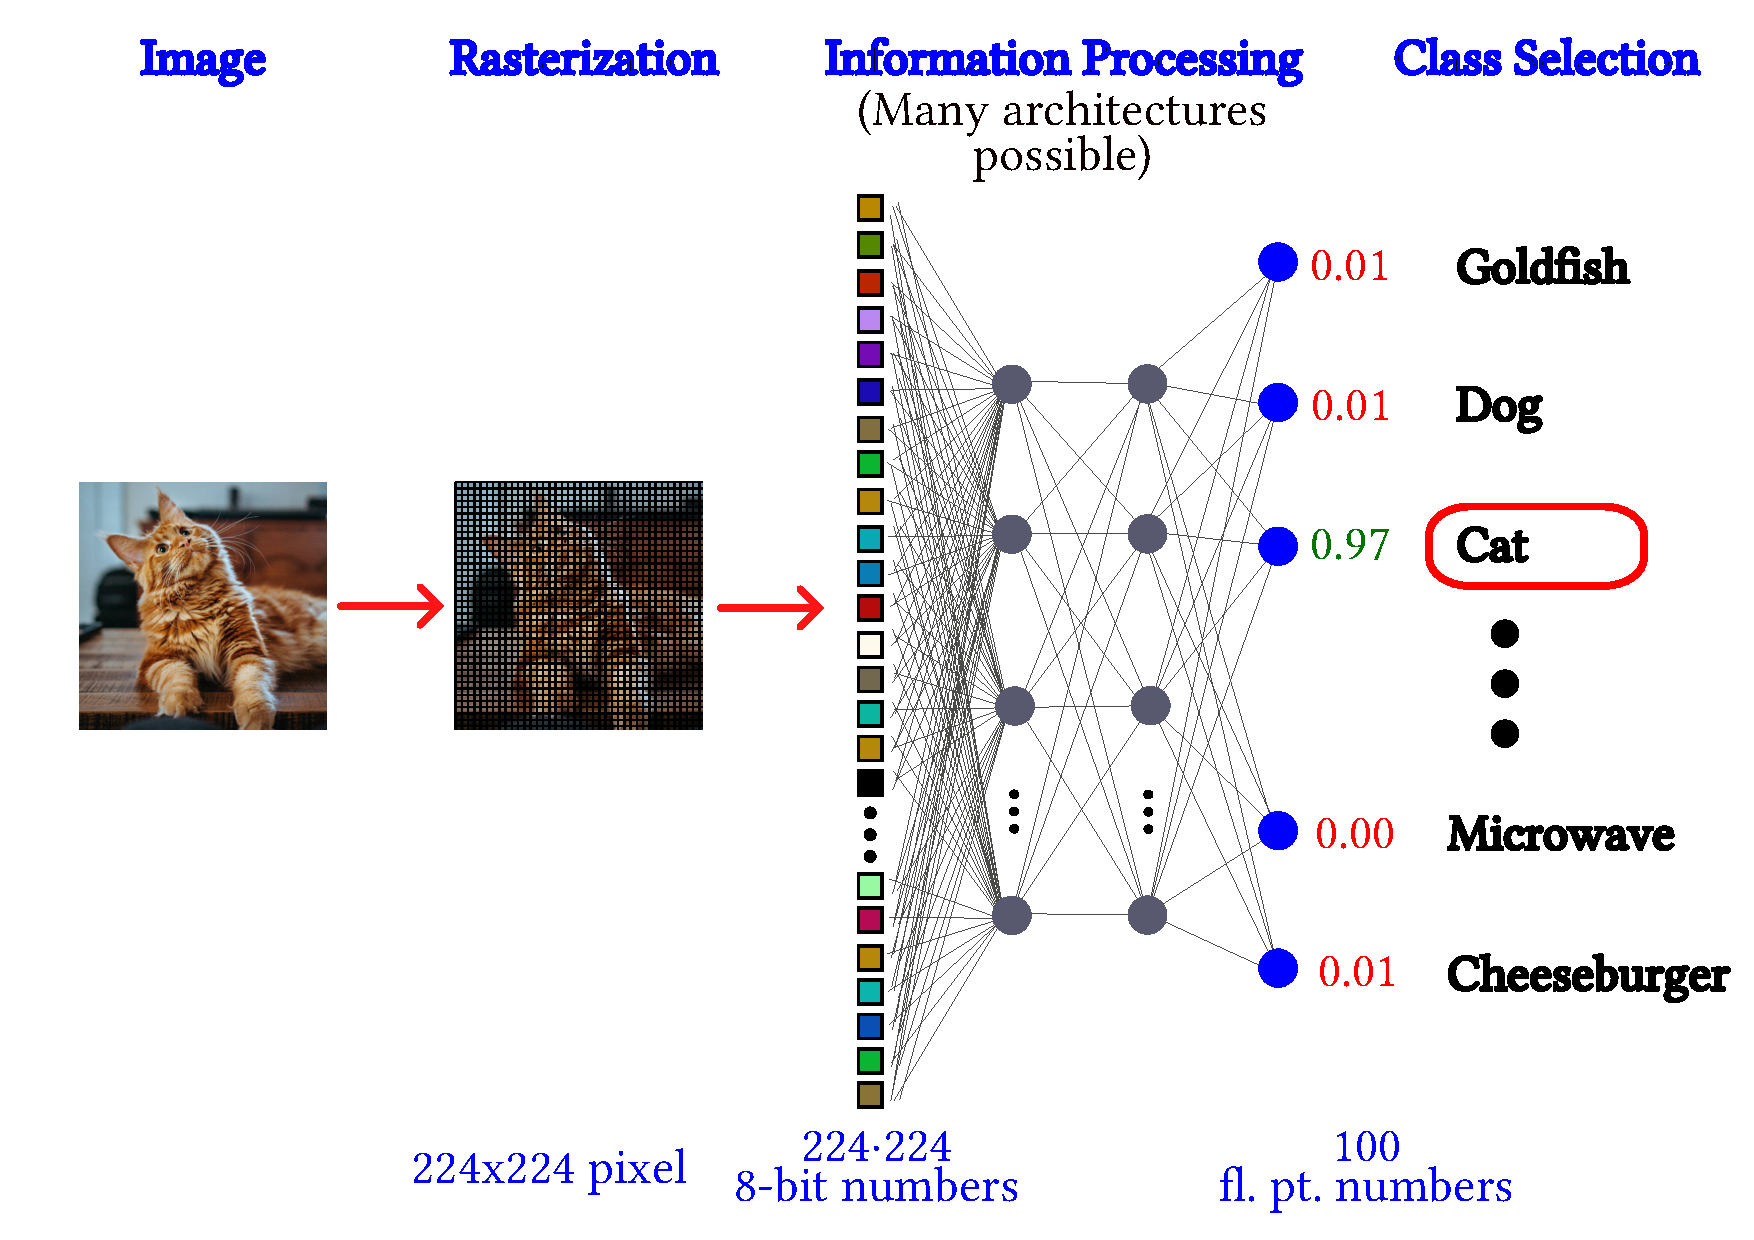
\includegraphics[width=\textwidth]{./theory/cs/image-classification/process.pdf}}
    \caption{Generalized schema of the image classification pipeline used in the experiments portion of this thesis.
        The image gets rasterized, resized to 224$\times$224 pixel and 8 bit color depth. Then the image is normalized, reshaped into vector form and processed from there. The MLP in this image is only a placeholder. Many of the later discussed neural network architectures treat the reshaping, casting and processing differently. The output for all networks needs to be in form of 100 floating point numbers. the one closest to one gets selected as the networks choice. The class name, the index represents can then be looked up.
        Cat image from \cite{catPhoto}.
    }
    \label{fig:immage-classification-general}
\end{figure}
